\documentclass[10pt]{article}
\usepackage{fancyhdr}
\usepackage{hyperref}
\usepackage{dirtree}
\usepackage[margin=0.6in]{geometry}
\usepackage{graphicx}

\hypersetup{
    colorlinks=true,
    linkcolor=blue,
    urlcolor=blue,
}

\title{Angry Birds: \\Shadow Flight}
\author{Piyush Prajapati \\ CS-104 Project}
\date{Spring 2023–24}

\pagestyle{fancy}
\lhead{Angry Birds: Shadow}
\rhead{Piyush Prajapati}

\begin{document}

\maketitle

\begin{abstract}
    This report documents the development of a Python game using Pygame. It explains the concept, design, implementation, key features, and how to play. The goal is to help readers understand the game without reading the source code.
\end{abstract}

\tableofcontents
\newpage

\section{Introduction}\label{sec:introduction}
In this game, players control a variety of birds with unique abilities launched at enemy towers. The goal is to launch birds from a slingshot with precise timing and angles to destroy the opposing team's tower while keeping your own safe. The game features turn-based mechanics, where each player takes their shot, aiming to cause maximum damage.

\section{Modules Used}\label{sec:modules}
The Python modules used are:
\begin{itemize}
    \item \texttt{pygame-ce} – For rendering graphics and handling events.
    \item \texttt{random} – For shuffling birds available to players at the start.
    \item \texttt{sys}, \texttt{os} – For system and file handling.
    \item \texttt{math} – For calculating distances and rotating birds based on direction.
\end{itemize}

\section{Directory Structure}\label{sec:directory-structure}
\dirtree{%
    .1 Root/.
    .2 main.py.
    .2 main game.py.
    .2 leaderboard.py.
    .2 load.py.
    .2 PlayerData.py.
    .2 settings.
    .2 tutorial.py.
    .2 Utils.py.
    .3 collision.py.
    .3 config.py. 
    .3 helper.py. 
    .2 assets/.
    .3 Images/.
    .3 Fonts/.
    .3 Sounds/.
    .2 data/.
    .3 lastgame.txt.
    .3 player.txt.
    .3 settings.txt.
    .3 Towers.txt.
    .2 Scenes/.
    .3 background.py.
    .3 main menu.py.
    .2 Entities/.
    .3 Birds and blocks.py.
    .3 slingshot.py.
    .3 Button.py.
}

The \texttt{Entities} directory contains classes for the slingshot, blocks, and bird types.\texttt{data/} stores text files representing game states.

\section{How to Run the Game}\label{sec:running-instructions}

\subsection{Prerequisites}
Ensure Python is installed. Then run:
\begin{verbatim}
pip install pygame-ce
python game.py
\end{verbatim}

If using traditional Pygame:
\begin{verbatim}
pip uninstall pygame
pip install pygame-ce
\end{verbatim}

\subsection{Game Navigation}
On running the main file, a main screen appears.
\begin{itemize}
    \item Click \texttt{New Game} to begin. If a previous game is saved, click \texttt{Load Previous}.
    \item Go to \texttt{Settings} to modify preferences or click \texttt{Tutorial} for instructions.
    \item Click \texttt{Quit} to exit or \texttt{Leaderboard} to view rankings.
    \item After starting a new game, enter your name and choose a tower. Then the second player will do the same.
    \item During gameplay, select a bird from the top menu and launch it by left-clicking and dragging on the slingshot.
    \item If super birds are enabled, birds have a power bar. Press \texttt{s} to activate their superpower once ready.
    \item Press \texttt{Esc} to pause the game—options include continue, restart, tutorial, and save.
    \item Games can be saved manually or autosaved when exiting.
\end{itemize}

\section{Game Screens}\label{sec:screens}

\subsection{Home Screen}
\begin{figure}[h!]
    \centering
    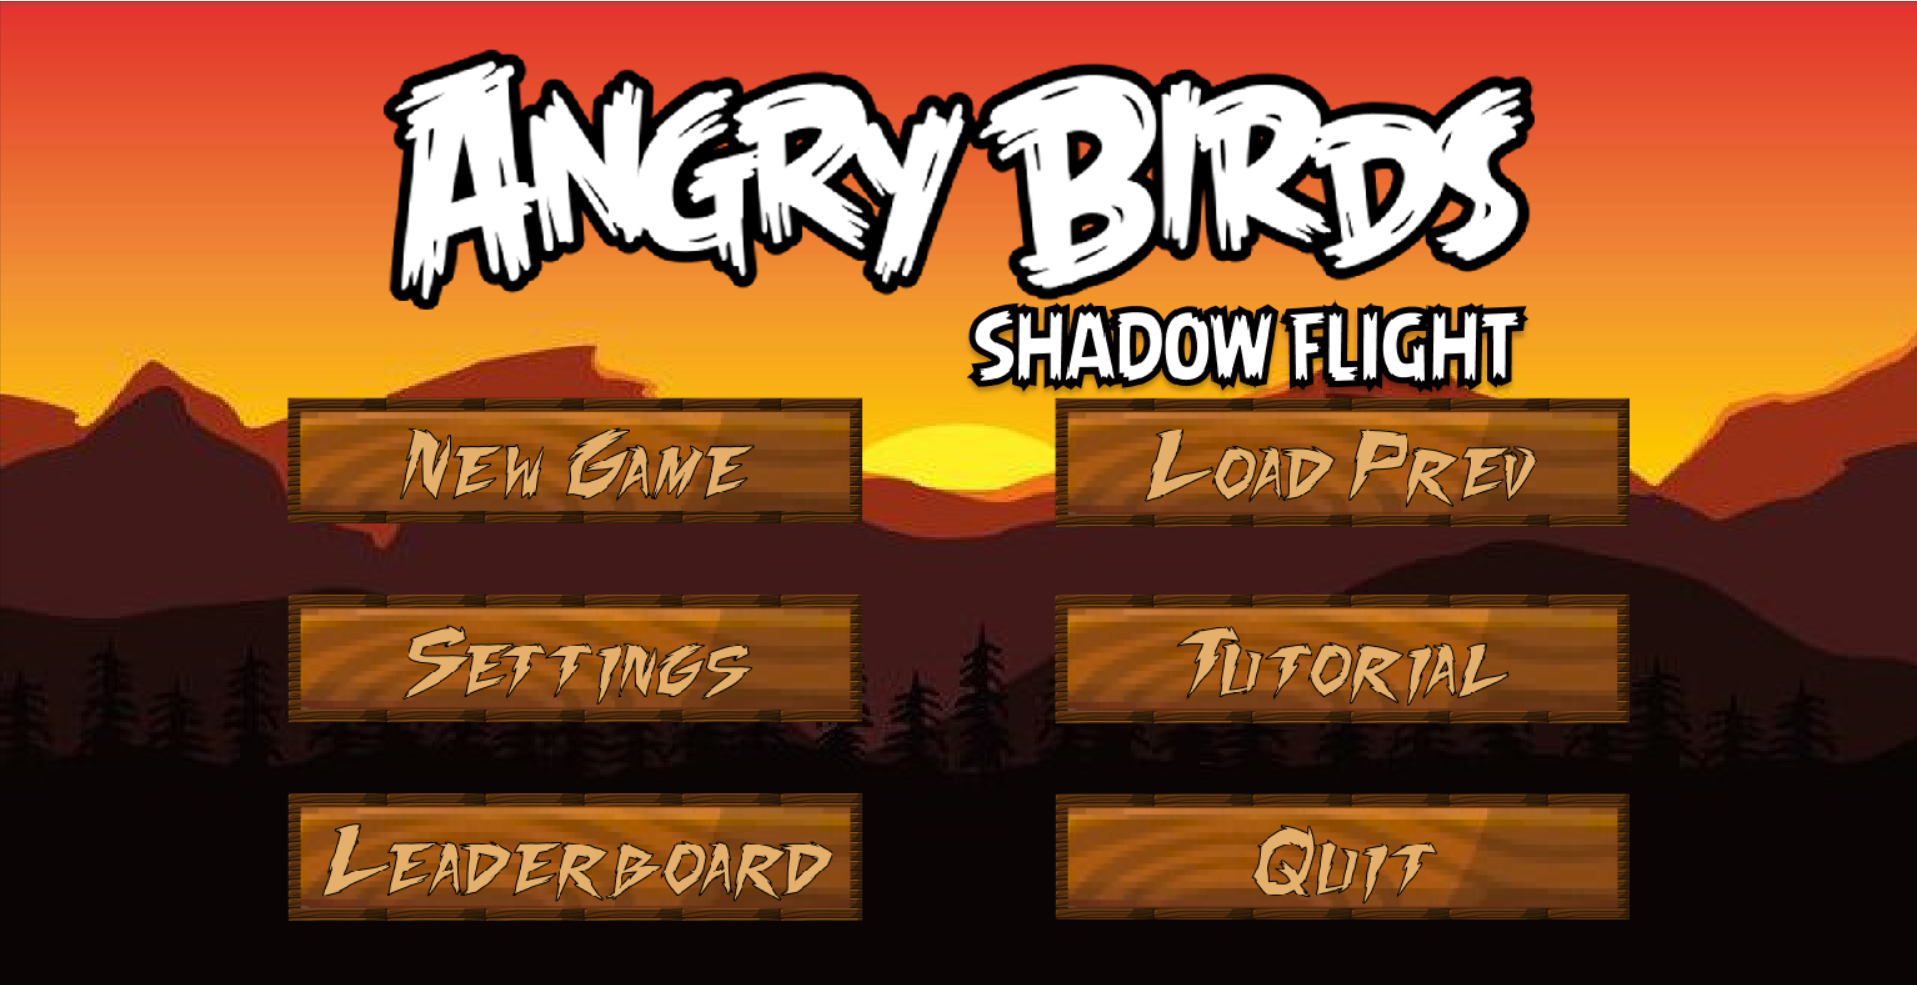
\includegraphics[width=0.5\textwidth]{home.png}
    \caption{Intro Screen}
\end{figure}

\subsection{Tower Selection}
\begin{figure}[h!]
    \centering
    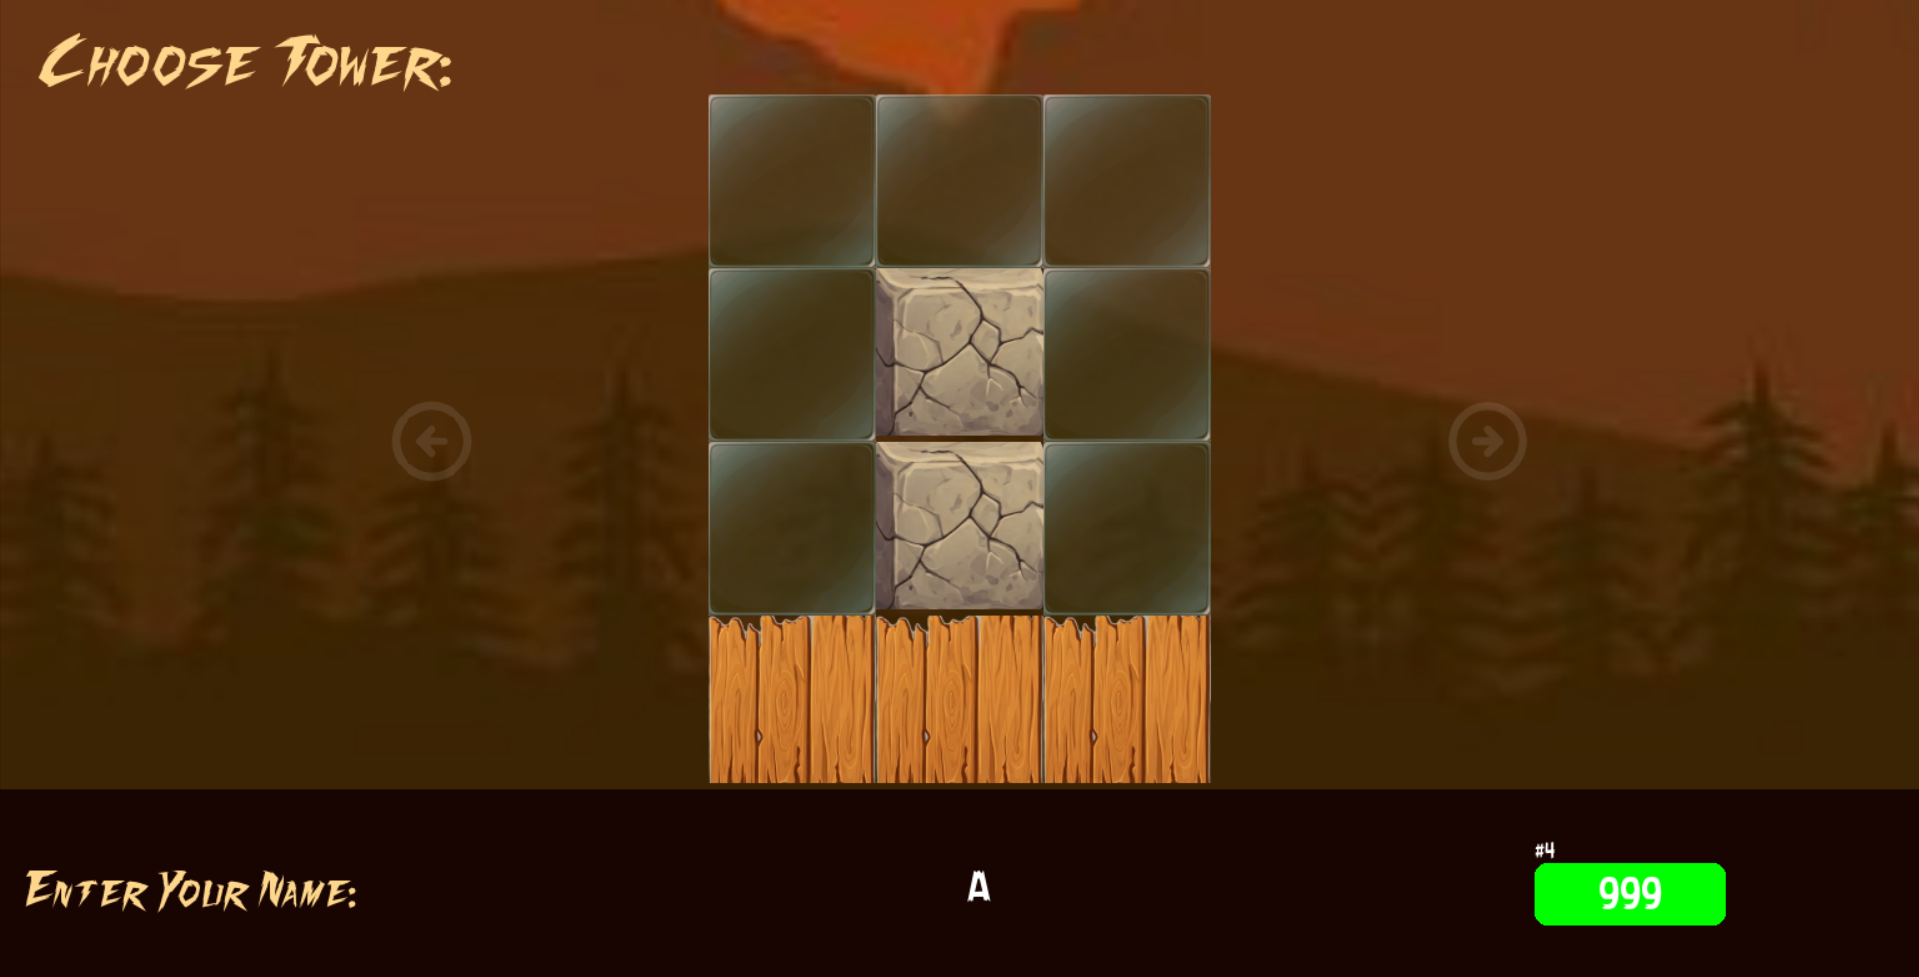
\includegraphics[width=0.5\textwidth]{selection.png}
    \caption{Main Menu}
\end{figure}

\subsection{In-Game Screenshot}
\begin{figure}[h!]
    \centering
    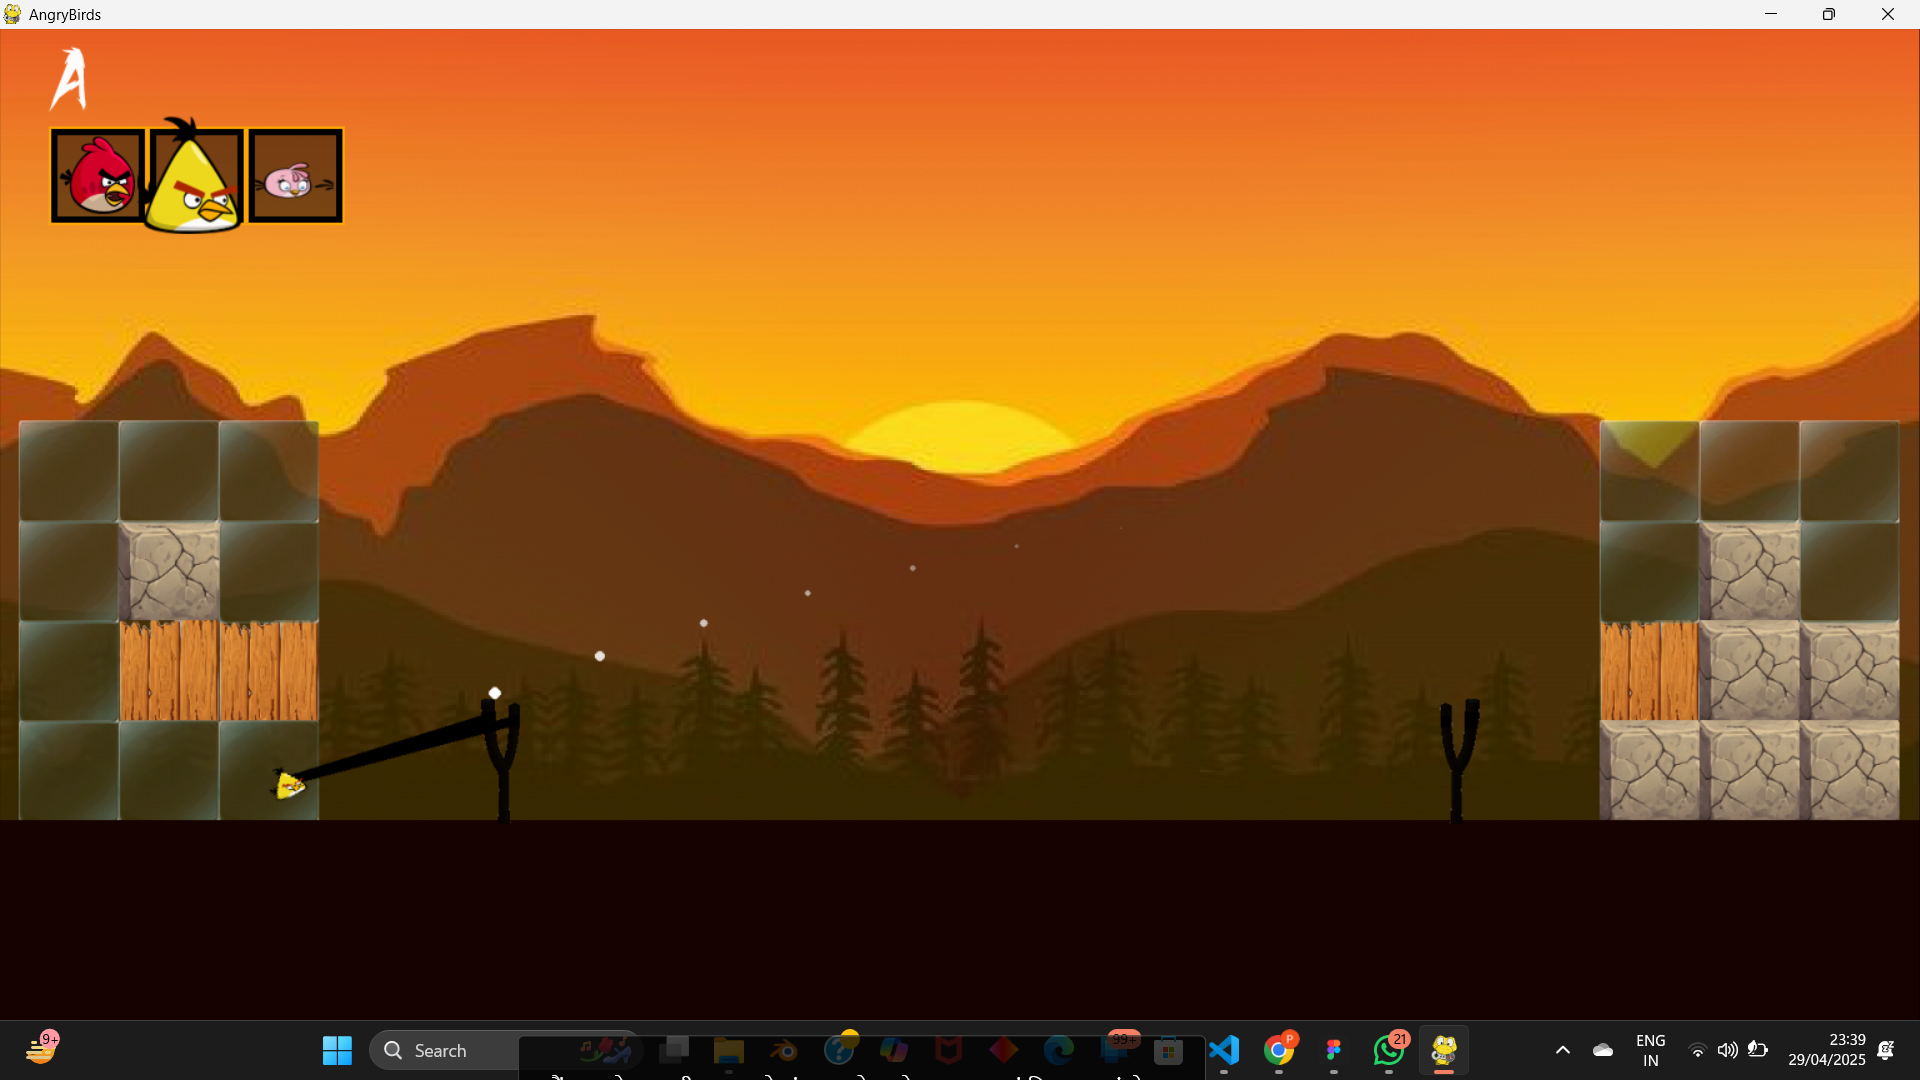
\includegraphics[width=0.5\textwidth]{game.png}
    \caption{Gameplay}
\end{figure}

\subsection{Pause Screen}
\begin{figure}[h!]
    \centering
    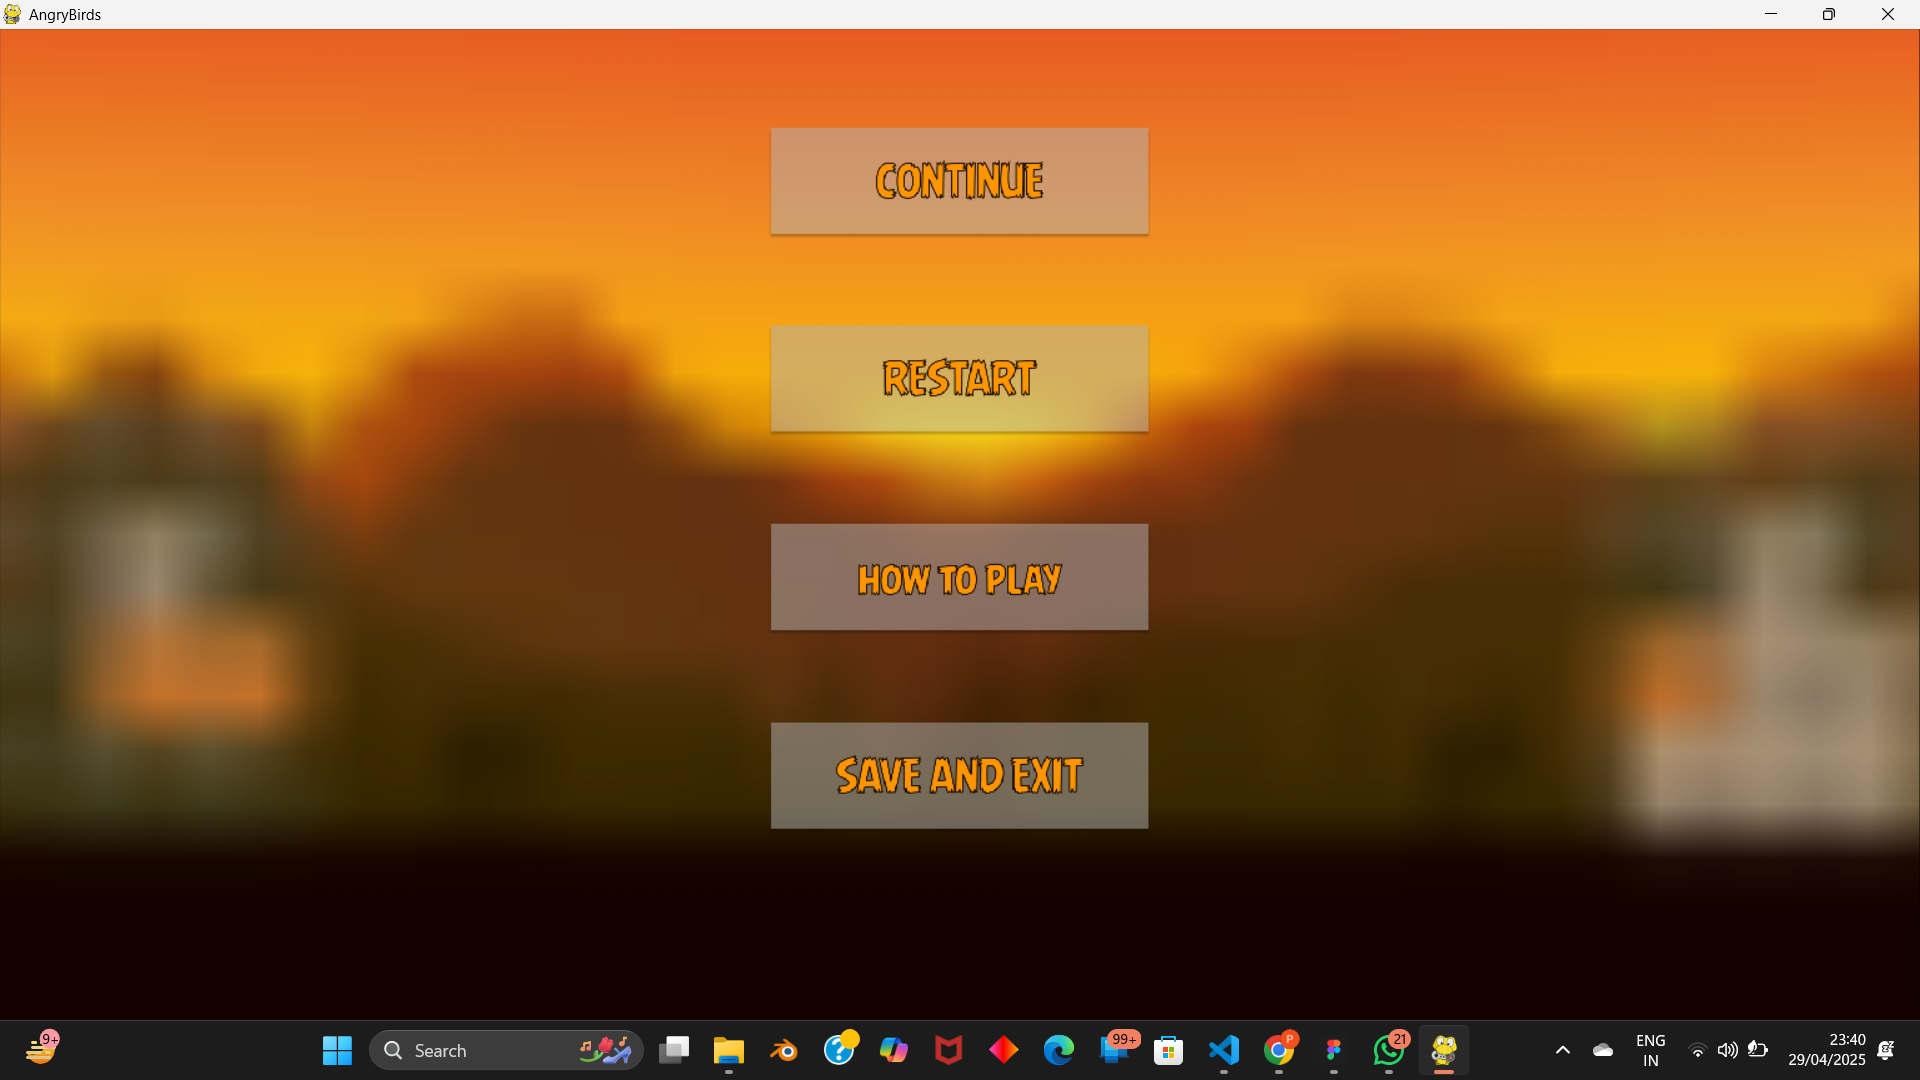
\includegraphics[width=0.5\textwidth]{pause.png}
    \caption{Pause Screen}
\end{figure}

\subsection{Leaderboard}
\begin{figure}[h!]
    \centering
    
\includegraphics[width=0.5\textwidth]{leaderboard.png}
    \caption{Leaderboard}
\end{figure}

\section{Implementation Details}\label{sec:implementation}
\begin{itemize}
    \item \textbf{Slingshot Logic:} Calculates relative position from mouse drag and converts to velocity.
    \item \textbf{Tower Collision:} Handled via custom functions in the \texttt{Entities} module.
    \item \textbf{Tower Damage:} Depends on bird properties and impact velocity.
    \item \textbf{Leaderboard:} Uses a basic Elo system to update rankings.
    \item \textbf{Save Logic:} Game state is stored and retrieved from text files.
    \item \textbf{Tower Selection:} First tower is user-selected; second is chosen with matching block count.
    \item \textbf{Bird Generation:} Player selects one of three birds each turn; the chosen bird is moved to the end of the queue.
    \item \textbf{Super Power Logic:} Birds gain energy to unlock superpowers, defined in their respective classes.
\end{itemize}

\section{Customization Features}\label{sec:features}
\begin{itemize}
    \item Sunset theme with authentic Angry Birds sound effects.
    \item Save/load game functionality and in-game tutorial with bird introductions and gameplay tips.
    \item Animations like fade-in, fade-out, and side pop-ups.
    \item Settings menu with volume and autozoom adjustments.
    \item Autozoom focuses on opponent's tower when a block is destroyed. Press \texttt{Space} to exit or disable it in settings.
    \item Birds have unique superpowers:
    \subsection*{Super Powers}
    \begin{itemize}
        \item \textbf{RED:} Heavy armor; damage radiates to nearby blocks.
        \item \textbf{Chuck:} Pierces through blocks, especially wood.
        \item \textbf{Blues:} Splits into three birds; strong against glass.
        \item \textbf{Bomb:} Explodes on impact; highly effective on rocks.
        \item \textbf{Stella:} Absorbs opponent tower health and heals own tower.
    \end{itemize}
    \item Leaderboard with dynamic ELO updates.
    \item Pause screen supports restart, tutorial access, save, and exit.
\end{itemize}

\section{Difficulties Faced}\label{sec:difficulties}
\begin{itemize}
    \item Modulating and organizing a large number of files was time-consuming and confusing initially.
    \item Finding suitable sprites and correct sound effects that matched the theme took significant effort.
    \item Designing all components and game logic from scratch required a lot of trial and error.
    \item Implementing accurate collision detection between birds, towers, and blocks was particularly challenging.
    \item Designing and implementing unique superpowers for each bird was conceptually and technically difficult.
    \item Creating smooth animations and transitions required precise timing and graphical logic.
    \item Building the player data entry and management screen with validation was a complex task.
\end{itemize}
\section{Future Improvements}\label{sec:future}
There are several features and upgrades I plan to implement in the future:

\begin{enumerate}
    \item \textbf{Custom Tower Builder:} Allow players to design their own tower layouts before the game starts. My current system is not hardcoded, and can support any tower shape or size. This feature will give players more creativity and control.
    
    \item \textbf{Ultimate Superpowers:} I have planned a set of ultimate superpowers for each bird, which are conceptually complete and pseudocoded mentally. Implementing them will take approximately two days.

    \item \textbf{Enhanced Music and Animations:} Add a richer set of background music tracks, dynamic sound effects, and smoother animations for actions like launching, collision, and bird powers.

    \item \textbf{Curved Terrain:} The current game has a flat ground. I plan to add collision logic for curved or irregular terrain to enhance realism and strategy.

    \item \textbf{Additional Birds:} Introduce more bird types with distinct abilities, strengths, and animations to increase game variety.

    \item \textbf{Custom Levels and Campaign Mode:} Include predefined levels or a level progression system where difficulty increases and players unlock birds/towers.
    \item \textbf{Power-up Drops and Pickups:} Add randomly spawning power-ups or traps to make gameplay less predictable.

    \item \textbf{Replays and Highlights:} Let players view replays of their launches and create short highlight clips.

    \item \textbf{Analytics and Stats Screen:} Track and display stats like hit accuracy, most used birds, damage dealt, etc.
\end{enumerate}

\section{References}
\begin{thebibliography}{9}
    \bibitem{pygameCEDoc}
    Pygame-CE Docs \\
    \url{https://pyga.me/docs/}

    \bibitem{gfg}
    Geeks for geeks tutorial blogs \\
    \url{https://www.geeksforgeeks.org/pygame-tutorial/}

    \bibitem{chatgpt}
    Chatgpt \\
    \url{https://chatgpt.com/?temporary-chat=true}
    \bibitem{gemini}
    gemini for sprite generation \\
    \url{https://gemini.google.com/app?hl=en-IN}
    \bibitem{pintererst}
    Pinterest for background image \\
    \bibitem{angrybirdsfandom}
    Angry birds fandom page \\
    \url{https://angrybirds.fandom.com/wiki/Slingshot}
    \bibitem{angrybirdsfandom}
    for sfx
    \url{https://www.myinstants.com}
    
\end{thebibliography}

\end{document}
